\appendix
\chapter*{Validation Test Results: RealSense D415}
\label{chap:rsd415}
%%%%%%%%%%%%%%%%%
%RealSense D-415
\begin{figure}[htp]
\begin{center}
{
  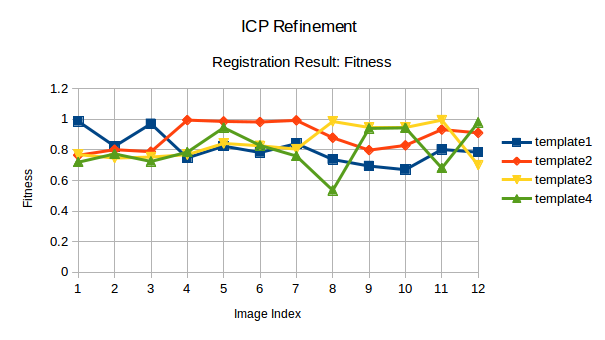
\includegraphics[clip,width=0.7\columnwidth]{figures/newreal_fitness.png}
}
\end{center}
\begin{center}
{
  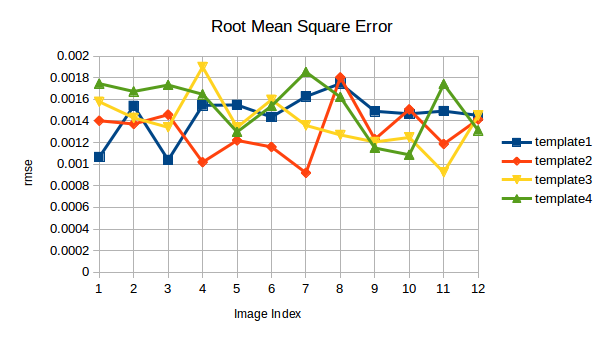
\includegraphics[clip,width=0.7\columnwidth]{figures/newreal_rmse.png}
}
\end{center}
\caption{Overview of the Validation Test: RealSense D-415}
\label{setupsystem1}
\end{figure}



\begin{table}[ht]
\renewcommand{\arraystretch}{1.3}
\caption{Absolute Error Values (RealSense D-415 Camera).}
\label{absolute}
\centering
\begin{tabular}{|c||c||c||c||c|}
\hline
  & Mean (2nd Exp )& STD \\
\hline
x-axis (cm) & 0.009 & 0.001
 \\
\hline
y-axis (cm) & 0.001 & 0.001  \\
\hline
yaw angle (degrees)& 0.698 & 0.400 \\
\hline
\hline
\end{tabular}
\end{table}

%%%%%%%%%%%%%%%%%%%%%%%%%%%%%%%%%%5
%RealSense D-415
\begin{figure}[htp]
\begin{center}
{
  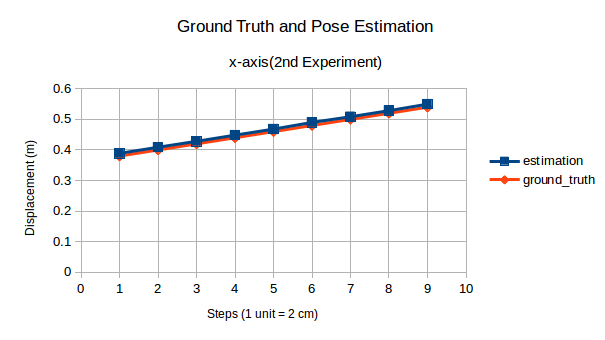
\includegraphics[clip,width=0.7\columnwidth]{figures/x_newrealsense.png}
}
\end{center}
\begin{center}
{
  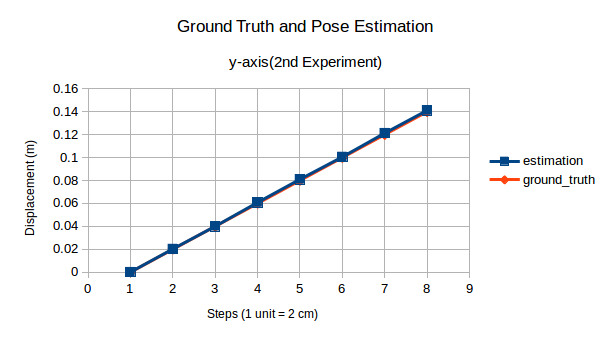
\includegraphics[clip,width=0.7\columnwidth]{figures/y_newrealsense.png}
}
\end{center}

\begin{center}
{
  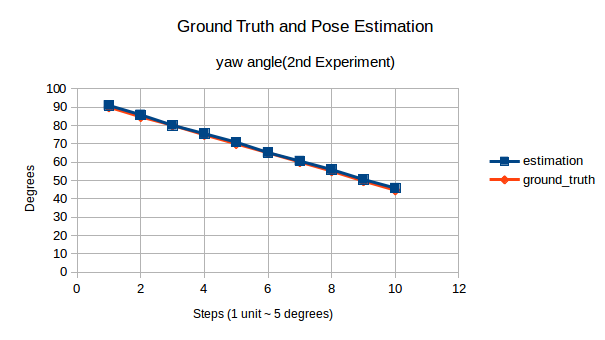
\includegraphics[clip,width=0.7\columnwidth]{figures/yaw_newrealsense.png}
}
\end{center}
\caption{Ground Truth and Pose Estimation ($2^{nd}$ Experiment, RealSense D-415}
\label{setupsystem1}
\end{figure}
